% Capítulo 8: cifra de César com chave 3, em duas faixas de 13 letras.
\documentclass[border=4pt]{standalone}
\usepackage[utf8]{inputenc}
\usepackage[T1]{fontenc}
% Estilo comum das figuras de vetores (capítulo 8).
\usepackage{tikz}
\usetikzlibrary{arrows.meta, positioning, calc, decorations.pathreplacing}
\definecolor{navy}{RGB}{23,45,80}
\definecolor{laranja}{RGB}{250,110,29}
\definecolor{cinzalogo}{RGB}{107,114,126}
\definecolor{azul}{RGB}{205,222,247}
\tikzset{
  casa/.style={draw=navy, line width=0.9pt, minimum width=8mm, minimum height=7mm,
               inner sep=0pt, font=\sffamily\small},
  pronta/.style={casa, fill=azul},
  parte/.style={casa, fill=laranja!12},
  marcada/.style={casa, fill=laranja!45, draw=laranja},
  fora/.style={casa, draw=cinzalogo!60, dashed, fill=white, text=cinzalogo!60},
  indice/.style={font=\sffamily\scriptsize, text=cinzalogo},
  explica/.style={font=\sffamily\small, text=navy, anchor=east},
  legenda/.style={font=\sffamily\scriptsize, text=cinzalogo},
  rotulo/.style={font=\sffamily\small\bfseries, text=navy},
  seta/.style={-{Stealth[length=2.2mm]}, navy, line width=0.9pt},
  chave/.style={decorate, decoration={brace, amplitude=4pt, mirror}, navy, line width=0.8pt},
}
% \vetor{nome}{x}{y}{valor/estilo, valor/estilo, ...}: casas lado a lado, chamadas nome0, nome1...
\newcommand{\vetor}[4]{%
  \foreach \valor/\estilo [count=\i from 0] in {#4} {
    \node[\estilo] (#1\i) at ($(#2, #3) + (\i*0.8, 0)$) {\valor};
  }
}

\tikzset{
  casa/.append style={minimum width=7mm, minimum height=7mm, font=\ttfamily\small},
  liga/.style={-{Stealth[length=1.6mm]}, cinzalogo, line width=0.5pt},
}
\begin{document}
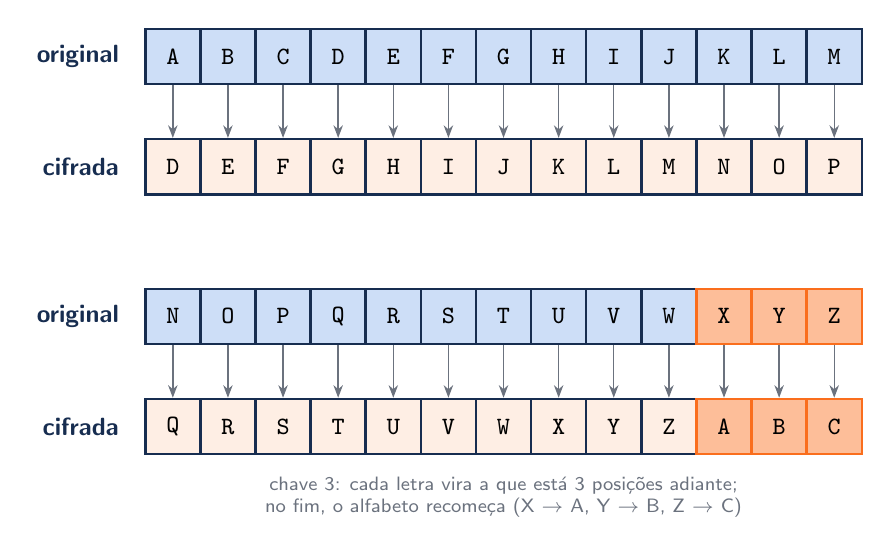
\begin{tikzpicture}[x=7mm]
  \foreach \l [count=\i from 0] in {A,B,C,D,E,F,G,H,I,J,K,L,M,N,O,P,Q,R,S,T,U,V,W,X,Y,Z} {
    \pgfmathtruncatemacro{\col}{mod(\i, 13)}
    \pgfmathsetmacro{\y}{\i < 13 ? 0 : -3.3}
    \pgfmathtruncatemacro{\d}{mod(\i + 3, 26)}
    \pgfmathsetmacro{\letra}{{"A","B","C","D","E","F","G","H","I","J","K","L","M","N","O","P","Q","R","S","T","U","V","W","X","Y","Z"}[\d]}
    \ifnum\i>22
      \node[marcada] (o\i) at (\col, \y) {\l};
      \node[marcada] (d\i) at (\col, \y - 1.4) {\letra};
    \else
      \node[pronta] (o\i) at (\col, \y) {\l};
      \node[parte] (d\i) at (\col, \y - 1.4) {\letra};
    \fi
    \draw[liga] (o\i.south) -- (d\i.north);
  }
  \foreach \y in {0, -3.3} {
    \node[rotulo, anchor=east] at (-0.8, \y) {original};
    \node[rotulo, anchor=east] at (-0.8, \y - 1.4) {cifrada};
  }
  \node[legenda, align=center] at (6, -5.6) {chave 3: cada letra vira a que está 3 posições adiante;\\no fim, o alfabeto recomeça (X $\rightarrow$ A, Y $\rightarrow$ B, Z $\rightarrow$ C)};
\end{tikzpicture}
\end{document}
